\documentclass[12pt,oneside]{article}

%%%%%%%%%%%%%%%%%%%%%%%%%%%%
%%   Additional packages  %%
%%%%%%%%%%%%%%%%%%%%%%%%%%%%
\usepackage{enumerate}
\usepackage{fancyhdr}
\usepackage{ifthen}
\usepackage{a4wide}
\usepackage{graphicx}
\usepackage{palatino}
\usepackage{multirow}
\usepackage{booktabs}
\usepackage{titlesec}
\usepackage{enumitem}% http://ctan.org/pkg/enumitem
\usepackage{amsmath}
\usepackage{tabularx}  % added for wide tables with line breaks
\usepackage{longtable} % added: the generative-AI table can break across pages
\usepackage[section]{placeins} % added: keeps figures and tables inside their section

\newboolean{englishLanguage}
%%%%%%%%%%%%%%%%%%%%%%%%%%%%%%%%%
%%%%%%%%%%%%%%%%%%%%%%%%%%%%%%%%%
%%% CHANGE true to false for a german paper %%%%
\setboolean{englishLanguage}{true}
%%%%%%%%%%%%%%%%%%%%%%%%%%%%%%%%%
%%%%%%%%%%%%%%%%%%%%%%%%%%%%%%%%%
\ifthenelse{\boolean{englishLanguage}}{\usepackage[ngerman, english]{babel}}{\usepackage[ngerman]{babel}}

\usepackage[T1]{fontenc}
\usepackage{paratype}\renewcommand{\familydefault}{\sfdefault}
\usepackage[utf8]{inputenc}
\usepackage[bookmarks]{hyperref}
\usepackage[justification=centering]{caption}
\usepackage[style=authoryear,natbib=true,backend=biber,maxbibnames=20]{biblatex}
\usepackage{csquotes}
\bibliography{literatur}
\setcounter{biburlnumpenalty}{9000}\setcounter{biburllcpenalty}{7000}\setcounter{biburlucpenalty}{8000} % allow line breaks in long URLs

\setlength{\parindent}{0em}
\setlist[itemize]{noitemsep, topsep=0pt}
\setlist[enumerate]{noitemsep, topsep=0pt}


%%%%%%%%%%%%%%%%%%%%%%%%%%%%%%
%% Definition of the header %%
%%%%%%%%%%%%%%%%%%%%%%%%%%%%%%

\pagestyle{fancy}
\fancyhf{}
\cfoot{\thepage}
\setlength{\headheight}{16pt}

%%%%%%%%%%%%%%%%%%%%%%%%%%%%%%%%%%%%%%%%%%%%%%%%%%%%%
%%  Definition of the cover page and title page  %%
%%%%%%%%%%%%%%%%%%%%%%%%%%%%%%%%%%%%%%%%%%%%%%%%%%%%%
% Only change to the template: the seal is included if seal.pdf exists
% (it comes with the official Overleaf template).
\newcommand{\JMUSeal}{\IfFileExists{seal.pdf}{\includegraphics[width=2in]{seal.pdf}}{\mbox{}}}

\ifthenelse{\boolean{englishLanguage}}{
%%% ENGLISH VERSION
\newcommand{\JMUTitle}[9]{

  \thispagestyle{empty}
  \vspace*{\stretch{1}}
  {\parindent0cm
  \rule{\linewidth}{.7ex}
  }
  \begin{flushright}
    \sffamily\bfseries\Huge
    #1\\
    \vspace*{\stretch{1}}
    \sffamily\bfseries\large
    #2\\
    \vspace*{\stretch{1}}
    \sffamily\bfseries\small
    #3
  \end{flushright}
  \rule{\linewidth}{.7ex}

  \vspace*{\stretch{1}}
  \begin{center}
    \JMUSeal \\
    \vspace*{\stretch{1}}
    \Large #5 \\

    \vspace*{\stretch{2}}
   \large Chair for Enterprise Artificial Intelligence\\
    \large Universität Würzburg\\
    \vspace*{\stretch{1}}
    \large Supervisor:  #8 \\[1mm]
    \large Assistant:  #9 \\[1mm]
    \vspace*{\stretch{1}}
    \large #6, #7
  \end{center}
}}{
%%% GERMAN VERSION
\newcommand{\JMUTitle}[9]{

  \thispagestyle{empty}
  \vspace*{\stretch{1}}
  {\parindent0cm
  \rule{\linewidth}{.7ex}
  }
  \begin{flushright}
    \sffamily\bfseries\Huge
    #1\\
    \vspace*{\stretch{1}}
    \sffamily\bfseries\large
    #2\\
    \vspace*{\stretch{1}}
    \sffamily\bfseries\small
    #3
  \end{flushright}
  \rule{\linewidth}{.7ex}

  \vspace*{\stretch{1}}
  \begin{center}
    \JMUSeal \\
    \vspace*{\stretch{1}}
    \Large #5 \\

    \vspace*{\stretch{2}}
   \large Lehrstuhl f\"ur K\"unstliche Intelligenz im Unternehmen\\
    \large Universität Würzburg\\
    \vspace*{\stretch{1}}
    \large Betreuer:  #8 \\[1mm]
    \large Assistent:  #9 \\[1mm]
    \vspace*{\stretch{1}}
    \large #6, den #7
  \end{center}
}}


\titlespacing*{\section}
{0pt}{3.5ex plus 1ex minus .2ex}{.2ex plus .2ex}
\titlespacing*{\subsection}
{0pt}{1.5ex plus 1ex minus .2ex}{.2ex plus .2ex}
\titlespacing*{\subsubsection}
{0pt}{1.5ex plus 1ex minus .2ex}{.2ex plus .2ex}

%%%%%%%%%%%%%%%%%%%%%%%%%%%%
%%  Beginning of the document  %%
%%%%%%%%%%%%%%%%%%%%%%%%%%%%


\begin{document}
    \ifthenelse{\boolean{englishLanguage}}{
    \JMUTitle
      {Forecasting German Day-Ahead Electricity Prices with Machine Learning}        % Title of the paper
      {Rashad Zarbaliyev, [Member 2], [Member 3]}                        % First and last name of the author
      {3288633, [Matriculation number], [Matriculation number]}

      {Project Report -- Practical Data Science (Winter Term 2026/27)} % Type of the work
      {W\"urzburg}                           % Place
      {18.01.2027}                          % Date of Submission
      {Prof. Dr. Gunther Gust}           % Name of the first examiner
      {Viet Nguyen} % Name of the supervisor
    }{\JMUTitle
      {Prognose deutscher Day-Ahead-Strompreise mit Machine Learning}        % Title of the paper
      {Rashad Zarbaliyev, [Mitglied 2], [Mitglied 3]}                        % First and last name of the author
      {3288633, [Matrikelnummer], [Matrikelnummer]}

      {Projektbericht -- Practical Data Science (WS 2026/27)} % Type of the work
      {W\"urzburg}                           % Place
      {18.01.2027}                          % Date of Submission
      {Prof. Dr. Gunther Gust}           % Name of the first examiner
      {Viet Nguyen} % Name of the supervisor
      }

  \clearpage

\lhead{}
\pagenumbering{Roman}
    \setcounter{page}{1}

\tableofcontents
\clearpage

\addcontentsline{toc}{section}{\listfigurename}
\listoffigures

\addcontentsline{toc}{section}{\listtablename}
\listoftables
\clearpage

\setlength{\parskip}{0.5em}


%%%%%%%%%%%%%%%%%%%%%%%%%%%%
%%  Short Summary   %%
%%%%%%%%%%%%%%%%%%%%%%%%%%%%
\lhead{Abstract}
\section*{Abstract}

We forecast the hourly German day-ahead electricity price for the next day. We use only official data from SMARD, the electricity market data platform of the Bundesnetzagentur. All 27 features are past prices, calendar information or official day-ahead forecasts of load, wind and solar power. No actual values of the forecast day enter the models. Two simple baselines serve as benchmarks: a seasonal naive forecast and a linear regression. We compare them with a random forest, a neural network and the simple average of the three learned models. We retrain every model monthly on the previous two years. We selected the final model on the validation year 2025, before we used the test data.

The final model is the equally weighted average of linear regression, random forest and neural network. On the test period January to November 2026, it reaches a mean absolute error (MAE) of 18.18\,EUR/MWh. This error is 45.3\,\% lower than that of the seasonal naive forecast. The final model also wins significantly more test days than every other model (sign test, $p < 0.001$). Because the best single model changes from month to month, the average is the most robust choice. The official wind and solar forecasts are not guaranteed to be published before the auction. Without them, the MAE rises to 29.38\,EUR/MWh, so these forecasts carry most of the predictive skill. Feature importance and a partial dependence plot show that the models learn the merit-order relationship between residual load and price. As an extension, a logistic regression detects 92.9\,\% of the negative-price hours of 2026 (PR-AUC 0.84). The main remaining weakness is the underestimation of extreme price spikes.

\textbf{Keywords:} electricity price forecasting, day-ahead market, random forest, forecast averaging, merit order, negative prices


%%%%%%%%%%%%%%%%%%%%%%%%%%%%
%%  Settings  %%
%%%%%%%%%%%%%%%%%%%%%%%%%%%%
\clearpage
\pagenumbering{arabic}
    \setcounter{page}{1}
\lhead{\nouppercase{\leftmark}}

%%%%%%%%%%%%%%%%%%%%%%%%%%%%
%%  Main Section  %%
%%%%%%%%%%%%%%%%%%%%%%%%%%%%

\section{Introduction} \label{Introduction}

In Germany, most electricity for the next day changes hands in the day-ahead auction. Every day at 12:00, market participants submit their bids. The auction then sets a price for each delivery period of the following day. These prices serve as the reference for many contracts and operational decisions. Utilities use them to plan the dispatch of their power plants, and traders build their positions on them. Battery operators decide when to charge and discharge, and flexible industrial consumers shift their demand to cheaper hours. Good price forecasts therefore have a direct economic value.

Yet forecasting these prices has become considerably harder in recent years. The share of wind and solar power has grown strongly. The last German nuclear power plants shut down in April 2023, and the energy crisis of 2021--2022 pushed prices to unprecedented levels. In our data, the hourly price ranges from $-500$ to 936\,EUR/MWh. The number of hours with negative prices grew from 211 in 2019 to 573 in 2025. A forecast that simply repeats yesterday's prices misses most of these dynamics.

\subsection{Problem statement}

We predict the hourly day-ahead price (EUR/MWh) of the bidding zone Germany/Luxembourg for each hour of day $D$. We make the forecast at noon on day $D-1$. It may therefore only use information that is available at that time (Section~\ref{sec:leakage} discusses one caveat). The task is a supervised regression problem on time-series data. Our main evaluation metric is the mean absolute error (MAE).

As an extension, we predict whether an hour will have a negative price. This binary classification problem matters to battery operators, flexible consumers and owners of renewable plants. For them, negative prices mean either a revenue opportunity or a cost.

\subsection{Research questions}

\begin{enumerate}
    \item \textbf{RQ1:} How accurately do machine learning models forecast hourly day-ahead prices from official SMARD data alone? How do they compare to a seasonal naive forecast and a linear regression?
    \item \textbf{RQ2:} How should we train models in a market that changes over time? How much history should we use, and which model type is most robust?
    \item \textbf{RQ3:} Which features drive the forecasts, and do the models learn economically meaningful relationships?
    \item \textbf{RQ4:} How well can negative-price hours be detected in advance?
\end{enumerate}

\subsection{Contributions}

\begin{itemize}
    \item A reproducible data pipeline that turns four SMARD files into 27 features without using any actual values of the forecast day.
    \item A comparison of simple and more flexible models from the course (linear regression, random forest, neural network and their average). The comparison uses a realistic setting with monthly retraining.
    \item A robustness check that quantifies how much the forecasts depend on the official wind and solar forecasts.
    \item An analysis of feature importance and partial dependence that recovers the merit-order curve from data.
    \item A classifier for negative-price hours and a small dashboard to inspect the forecasts.
\end{itemize}

The remainder of this report proceeds as follows. Section~\ref{sec:related} reviews related work. Section~\ref{sec:data} describes the data and the exploratory analysis, and Section~\ref{sec:method} sets out the methodology. Section~\ref{sec:results} presents the results, and Section~\ref{sec:discussion} discusses errors, explanations and limitations. Section~\ref{sec:conclusion} concludes.

\section{Related Work} \label{sec:related}

\textbf{Electricity price forecasting.} \citet{weron2014} reviews roughly 15 years of methods for electricity price forecasting (EPF), from statistical time-series models to neural networks. He also discusses their strengths and weaknesses. He calls for comparative studies with the same datasets, robust error measures and a careful check of whether one model really outperforms another. We follow these recommendations in three ways. We use an official, public dataset and the MAE as main metric. We also compare the errors day by day with a simple significance test.

\textbf{Benchmarks and best practices.} \citet{lago2021} note that studies often compare new EPF methods on non-public datasets and on short test periods limited to one market. As a result, it remains unclear which methods work best. The authors propose guidelines for EPF research and review state-of-the-art algorithms. They also publish an open-access benchmark with two open-source forecasting models. They recommend a test period of at least one year and comparisons against simple benchmarks. Our test period covers ten and a half months (January to mid-November 2026). Together with the validation year 2025, we evaluate every model out-of-sample with monthly retraining on almost two years of data.

\textbf{Model structure and regularization.} \citet{ziel2018} study 12 power markets with 32 regression models estimated via the lasso. They find that shrinkage brings significant accuracy gains over commonly used EPF models. Moreover, no single model structure performs best across all datasets, seasons and hours. This finding supports our comparison of several model types and our hour-by-hour error analysis.

\textbf{Forecast combination.} \citet{nowotarski2014} compare schemes for averaging electricity price forecasts. Combining forecasts generally improves accuracy. Equally weighted averaging is a simple but powerful choice when no single model consistently outperforms the others. Our final model applies exactly this equal-weight averaging.

\textbf{Machine learning methods.} Random forests \citep{breiman2001} combine many decision trees. Each tree grows on a random sample of the data and considers a random selection of features at each split. We implement all models with scikit-learn \citep{pedregosa2011}, the library used throughout the course. Partial dependence plots \citep{friedman2001} reveal how a feature affects the forecasts of a complex model. They show the average forecast when one feature changes and all others keep their observed values.

\textbf{Our contribution.} Most of the studies above use data from before 2020. We study the German market from October 2018 to November 2026. This period includes the energy crisis, the nuclear phase-out and the switch to 15-minute products. We evaluate how simple models cope with such changes through monthly retraining.

\section{Data} \label{sec:data}

\subsection{Sources}

All data comes from SMARD, the electricity market data platform of the Bundesnetzagentur (Federal Network Agency) \citep{smard2026}. SMARD publishes it under the CC BY 4.0 licence, which permits free use with attribution. We downloaded four files with the settings country Germany, resolution hour, period 01.10.2018 to 17.11.2026 (Table~\ref{tab:files}). Each file has 71,281 hourly rows. We added nationwide public holidays with the Python package \texttt{holidays}, which contains the official German holiday dates.

\begin{table}[!htbp]
    \centering
    \caption{SMARD files used in this project}
    \begin{tabularx}{\textwidth}{lXl}
        \toprule
        SMARD file & Variables used & Role \\
        \midrule
        Day-ahead prices & Price of the bidding zone Germany/Luxembourg (EUR/MWh) & Target \\
        Forecasted consumption & Grid load and residual load forecasts (MWh) & Features \\
        Forecasted generation day-ahead & Wind onshore, wind offshore and solar forecasts (MWh) & Features \\
        Actual generation & Generation by energy source (MWh) & EDA only \\
        \bottomrule
    \end{tabularx}
    \label{tab:files}
\end{table}

The period starts on 1 October 2018. On that date, the joint German-Austrian bidding zone was split and the current German-Luxembourg zone began. The residual load equals the load minus wind and solar generation. In other words, it is the demand that conventional power plants have to cover.

\subsection{Data preparation}

One module, \texttt{src/data\_pipeline.py}, implements all preparation steps, and every notebook uses it. This makes the analysis reproducible from the raw files.

\begin{itemize}
    \item \textbf{Time index.} SMARD reports local time. At the switch to summer time one hour is missing; at the switch to winter time one hour appears twice. Because all files contain exactly one row per hour, we rebuild a clean UTC index and convert it to German time. A check of 26 October 2025 confirms the result: the repeated hour 02:00 is kept once in summer time and once in winter time.
    \item \textbf{Alignment.} The pipeline checks that all four files have identical timestamps row by row.
    \item \textbf{Missing values.} The consumption forecast is missing for one full day (31 January 2020, 24 hours). We fill this gap with the forecast of the same hour one week earlier, which has the same weekday profile. All other gaps only affect columns we do not use. Examples are nuclear generation after the phase-out and prices of the former German-Austrian zone.
    \item \textbf{15-minute products.} Since 1 October 2025, the day-ahead auction has traded 15-minute products. SMARD's hourly values are averages of the quarter-hours, so the hourly series remains consistent over the whole period.
\end{itemize}

After we build the lagged features (Section~\ref{sec:method}), we drop the first 30 days. This leaves 70,538 hourly observations.

\subsection{Exploratory data analysis}

\textbf{Price development.} Table~\ref{tab:yearly} and Figure~\ref{fig:daily} show strong changes over time. Prices were low and stable in 2019--2020. They rose to an average of 235\,EUR/MWh in the energy crisis of 2022 and then settled at a new, higher level. 2026 is more expensive (mean 121\,EUR/MWh) and more volatile than 2024--2025. With the growth of renewables, negative prices became much more frequent.

\begin{table}[!htbp]
    \centering
    \caption{Day-ahead price statistics by year (EUR/MWh; 2018 and 2026 are partial years)}
    \begin{tabular}{lrrrrr}
        \toprule
        Year & Mean & Std.\ dev. & Min & Max & Negative hours \\
        \midrule
        2018 (Oct--Dec) & 52.6 & 18.6 & $-19.4$ & 128.3 & 27 \\
        2019 & 37.7 & 15.5 & $-90.0$ & 121.5 & 211 \\
        2020 & 30.5 & 17.5 & $-83.9$ & 200.0 & 298 \\
        2021 & 96.8 & 73.7 & $-69.0$ & 620.0 & 139 \\
        2022 & 235.4 & 142.8 & $-19.0$ & 871.0 & 69 \\
        2023 & 95.2 & 47.6 & $-500.0$ & 524.3 & 301 \\
        2024 & 78.5 & 52.7 & $-135.4$ & 936.3 & 457 \\
        2025 & 89.3 & 52.1 & $-250.3$ & 583.4 & 573 \\
        2026 (Jan--Nov) & 121.0 & 76.3 & $-499.0$ & 697.3 & 462 \\
        \bottomrule
    \end{tabular}
    \label{tab:yearly}
\end{table}

\begin{figure}[!htbp]
    \centering
    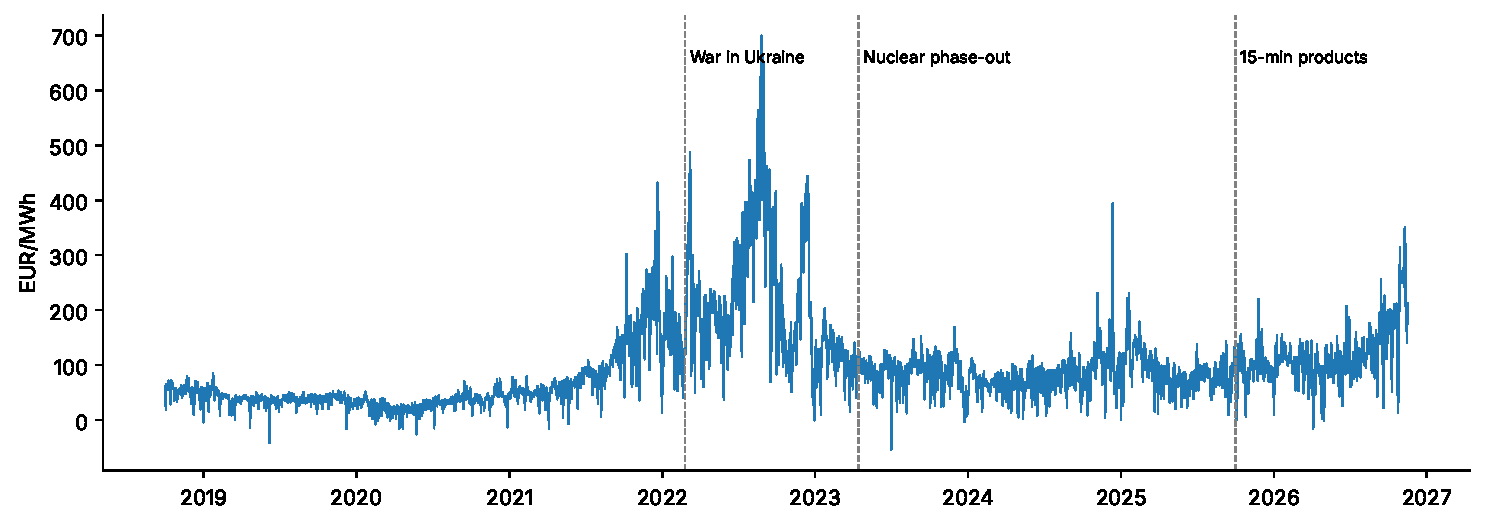
\includegraphics[width=\textwidth]{figures/fig_daily_price.pdf}
    \caption{Daily average day-ahead price (EUR/MWh) with major market events}
    \label{fig:daily}
\end{figure}

\textbf{Seasonality.} Prices follow a strong daily profile with a morning and an evening peak (Figure~\ref{fig:profile}). Since 2019, the growth of solar generation has made the midday hours much cheaper relative to the rest of the day. This creates a pronounced dip at noon. Prices are also lower on weekends and public holidays. On workdays in 2024--2026, the average price was about 105\,EUR/MWh on normal days and about 55\,EUR/MWh on public holidays.

\begin{figure}[!htbp]
    \centering
    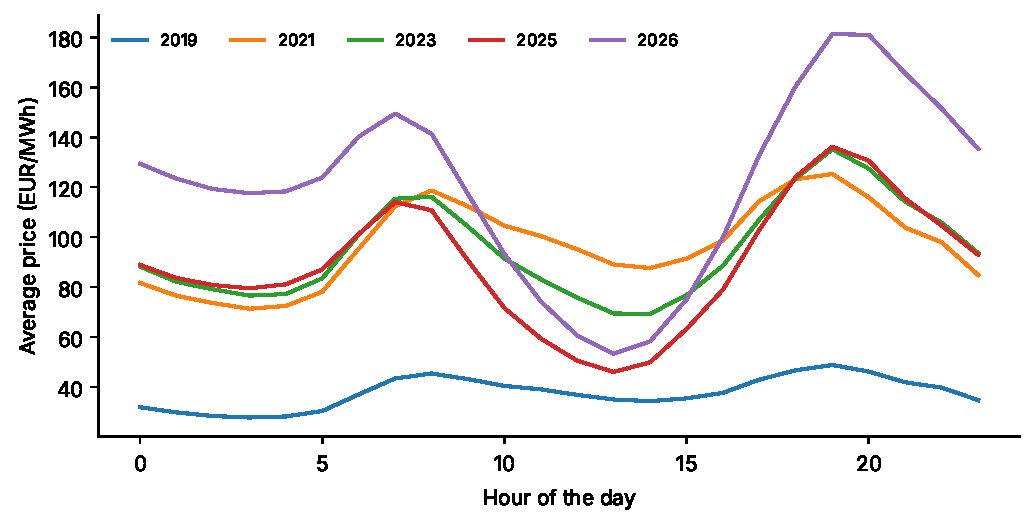
\includegraphics[width=0.62\textwidth]{figures/fig_daily_profile.pdf}
    \caption{Average price by hour of the day for selected years}
    \label{fig:profile}
\end{figure}

\textbf{Price drivers.} The forecasted residual load is the strongest fundamental driver of the price, with a correlation of 0.73 in 2024--2026. Solar ($-0.45$) and wind ($-0.30$) forecasts lower the price. Total load alone, by contrast, is only weakly related (0.18). Figure~\ref{fig:merit} shows an increasing, non-linear relationship between residual load and price. Between 2019 and 2025, the whole curve shifted upwards because of higher fuel and CO$_2$ costs. It also extends further to the left, since more hours have a particularly low residual load. When the forecasted renewable share exceeds 100\,\% of the load, 72\,\% of the hours have negative prices. For a share between 80\,\% and 100\,\%, the figure is 32\,\%.

\begin{figure}[!htbp]
    \centering
    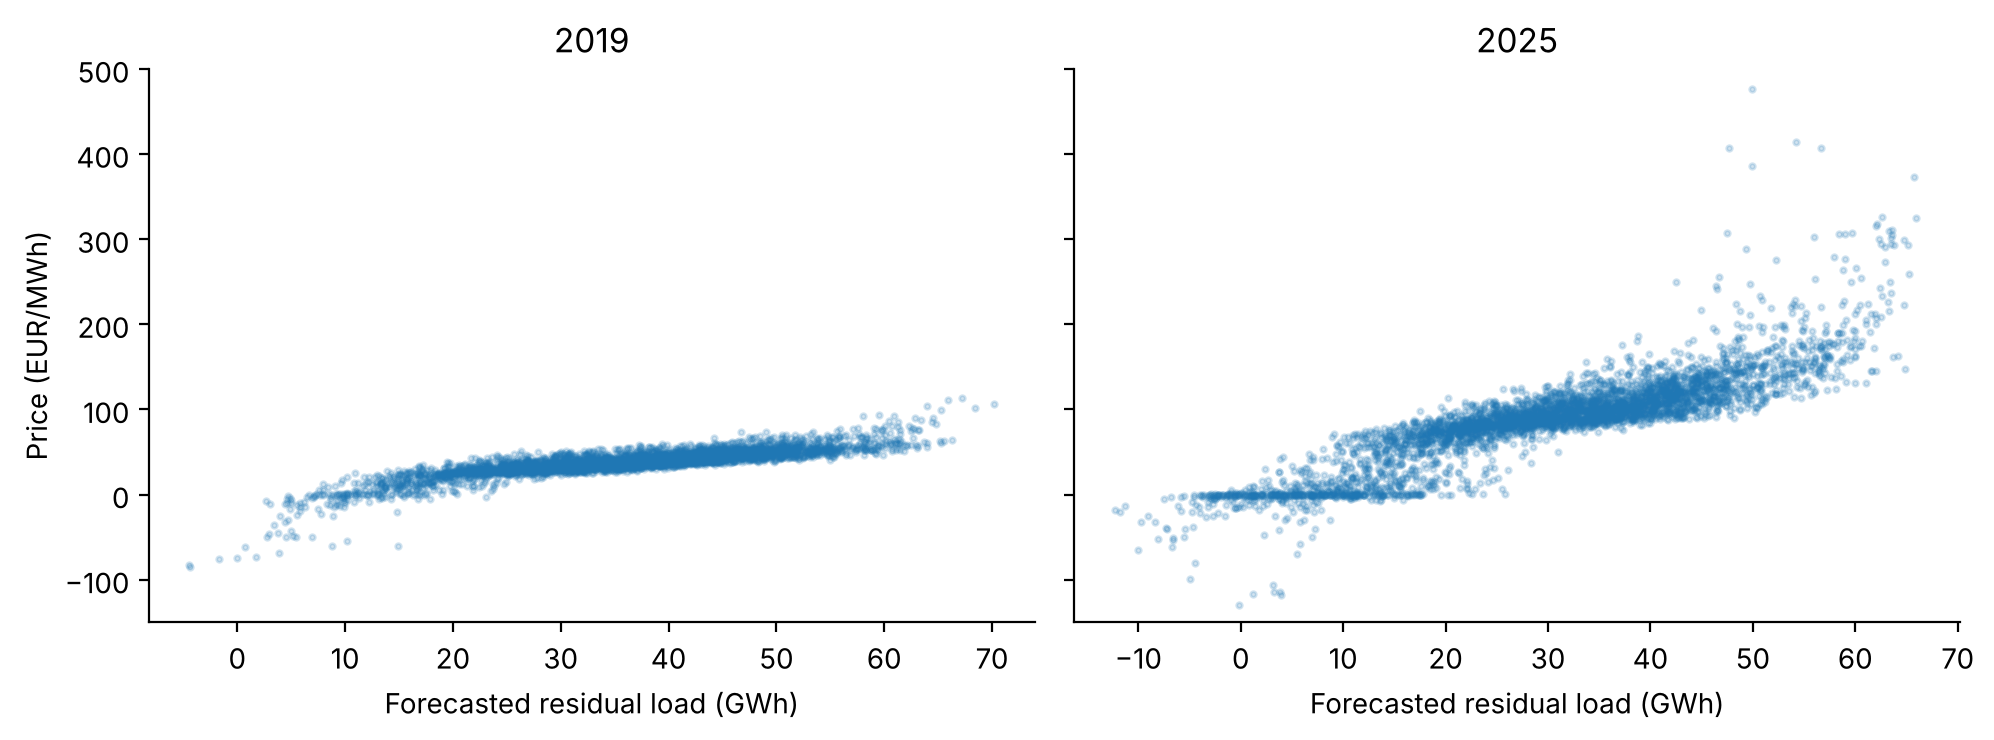
\includegraphics[width=\textwidth]{figures/fig_merit_order.png}
    \caption{Price vs.\ forecasted residual load in 2019 and 2025 (4,000 sampled hours each)}
    \label{fig:merit}
\end{figure}

\textbf{Generation mix.} The actual generation data (Figure~\ref{fig:mix}) reveals the structural change behind these patterns. The renewable share of generation rose from 42.8\,\% in 2019 to 58.9\,\% in 2025. Nuclear power disappeared in April 2023, and solar generation grew from 42\,TWh to 74\,TWh.

\begin{figure}[!htbp]
    \centering
    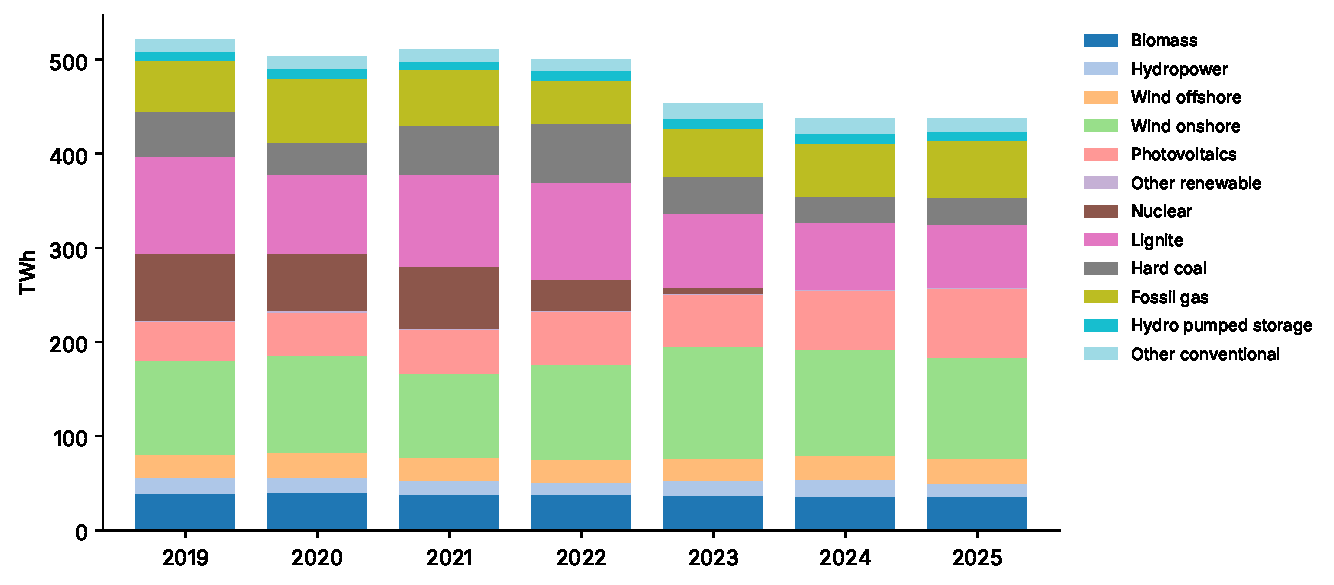
\includegraphics[width=0.72\textwidth]{figures/fig_generation_mix.pdf}
    \caption{Annual electricity generation in Germany by source (TWh)}
    \label{fig:mix}
\end{figure}

\textbf{Autocorrelation.} The autocorrelation of hourly prices has clear peaks at lags of 24 and 168 hours. These lags correspond to the same hour on the previous day and in the previous week. Since the prices of the forecast day itself are unknown at noon on day $D-1$, only lags of at least 24 hours are usable.

\textbf{Implications.} The EDA leads to five modeling decisions. (1) Train on recent data and retrain regularly, because the price level shifts. (2) Compare a linear model with models that can learn the non-linear merit-order relationship (random forest, neural network). (3) Include calendar features for daily, weekly and holiday patterns. (4) Include lagged prices of at least 24 hours. (5) Treat negative prices as a separate classification task.

\section{Methodology} \label{sec:method}

\subsection{Leakage rule} \label{sec:leakage}

The auction for day $D$ closes at 12:00 on day $D-1$. A feature for an hour of day $D$ is therefore only allowed if it is known at that time. This rule excludes two variables that would otherwise look highly useful. The first is the prices of neighbouring countries, which the same auction determines. The second is actual generation, which is published only afterwards. The rule allows SMARD's day-ahead forecasts for day $D$ and calendar information. It also allows all prices up to and including day $D-1$, which the auction on day $D-2$ set.

One caveat concerns the publication times of the forecasts. The transmission system operators must publish the day-ahead load forecast at least two hours before the auction closes. For the day-ahead wind and solar forecasts, however, the deadline is 18:00 on day $D-1$ \citep{eu2013transparency}. The wind and solar forecasts, and therefore the residual load, are thus not guaranteed to be available at noon. We use them as a proxy for the weather-based wind and solar forecasts that market participants prepare or buy themselves before the auction. If such forecasts are less accurate than the official ones, our errors are optimistic. Section~\ref{sec:robust} quantifies the worst case without any wind and solar information.

\subsection{Features}

We build 27 features in three groups (Table~\ref{tab:features}). Each feature is a short pandas operation in \texttt{src/\allowbreak data\_\allowbreak pipeline.py}. We shift all rolling statistics by 24 hours, so they only use prices up to day $D-1$.

\begin{table}[!htbp]
    \centering
    \caption{Model features}
    \begin{tabularx}{\textwidth}{lXX}
        \toprule
        Group & Features & Idea \\
        \midrule
        Fundamentals (11) & Load, residual load, wind onshore, wind offshore and solar forecasts; renewable share; residual load ramp (change to the previous hour); residual load relative to the daily mean; daily maximum and minimum of residual load; change of residual load vs.\ the same hour of the previous day & Merit order: the residual load determines which power plants set the price \\
        \midrule
        Calendar (6) & Hour, weekday, month, day of year, weekend flag, public holiday flag & Daily, weekly and seasonal demand patterns \\
        \midrule
        Past prices (10) & Price 24, 48 and 168 hours earlier; mean of the same hour over the last 7 days; mean, minimum and maximum of the previous day; 7-day and 30-day rolling mean; 7-day rolling standard deviation & Persistence and current price level (proxy for fuel and CO$_2$ costs, which are not in SMARD) \\
        \bottomrule
    \end{tabularx}
    \label{tab:features}
\end{table}

\subsection{Data split}

Time series must not be split randomly, because the model would then learn from the future. Instead, we use three consecutive periods (Table~\ref{tab:split}). The training period starts after the energy crisis, because the price dynamics of 2021--2022 no longer represent the current market. Section~\ref{sec:window} provides evidence for this choice.

\begin{table}[h!]
    \centering
    \caption{Chronological data split}
    \begin{tabular}{llrl}
        \toprule
        Set & Period & Hours & Purpose \\
        \midrule
        Training & Jan 2023 -- Dec 2024 & 17,544 & Fit the models \\
        Validation & Jan 2025 -- Dec 2025 & 8,760 & Choose the window and the final model \\
        Test & Jan 2026 -- 17 Nov 2026 & 7,704 & Final evaluation, used once \\
        \bottomrule
    \end{tabular}
    \label{tab:split}
\end{table}

\subsection{Models}

All models come from scikit-learn \citep{pedregosa2011}, and the course introduced each of them.

\begin{itemize}
    \item \textbf{Seasonal naive (baselines).} The price at the same hour one day (\texttt{lag24}) or one week (\texttt{lag168}) earlier. Any useful model must beat this.
    \item \textbf{Linear regression (interpretable baseline).} Ordinary least squares on all 27 standardized features.
    \item \textbf{Random forest} \citep{breiman2001}. 200 trees, at least 5 samples per leaf, 50\,\% of the features considered at each split. Trees can learn non-linear effects such as the merit-order curve.
    \item \textbf{Neural network (MLP).} A multi-layer perceptron with two hidden layers (128 and 64 neurons) on standardized features. It uses early stopping on 10\,\% of the training data.
    \item \textbf{Average of the three models.} The forecast is the plain mean of the linear regression, random forest and MLP forecasts. We estimate no weights, following the finding of \citet{nowotarski2014} that simple averaging is robust.
\end{itemize}

We set the hyperparameters of the random forest and the MLP to common values and did not tune them systematically. This keeps the comparison simple; Section~\ref{sec:limitations} discusses it as a limitation.

\subsection{Monthly retraining} \label{sec:rolling}

In practice, forecasters retrain their models regularly with the newest data. We simulate this with a simple loop. For each month of the evaluation period, we retrain every model on the preceding $N$ days. Each model then predicts all hours of that month. We chose the window length $N$ on the validation year (Section~\ref{sec:window}). The test year follows the same procedure, so the test results reflect how the models would have performed in real use.

\subsection{Evaluation metrics}

\begin{itemize}
    \item \textbf{MAE} (main metric): the mean absolute error in EUR/MWh. It is easy to interpret and robust to single extreme hours.
    \item \textbf{RMSE}: penalizes large errors more strongly.
    \item \textbf{MAE on extreme hours}: the error on the 5\,\% highest-priced hours (spikes) and on hours with negative prices.
\end{itemize}

We do not use percentage errors such as the MAPE, because prices close to or below zero make them meaningless.

A lower average error can come from a few days on which one model was lucky. We therefore also compute each model's MAE for every single test day. We then count the days on which the final model is more accurate than each other model. If two models were equally good, each would win about half of the days, like a coin flip. A sign test, i.e.\ a binomial test of the number of days won against 50\,\%, builds on this idea. It gives the probability of a result at least this extreme under that assumption. We call a difference significant if this p-value is below 0.05.

\subsection{Extension: negative-price classification} \label{sec:classmethod}

The target is 1 if the price is below 0\,EUR/MWh and 0 otherwise. Only about 6\,\% of the hours are negative, so accuracy would be misleading. A model that never predicts a negative price would be 94\,\% accurate. We therefore report the area under the precision-recall curve (PR-AUC, main metric), precision, recall and F1. We compare three approaches. The first is a simple rule: predict \enquote{negative} if the forecasted renewable share exceeds a threshold chosen on the training data. The others are a logistic regression and a random forest with 300 trees. For each model, we keep the decision threshold that maximizes F1 on the validation year fixed for the test. For the test, we retrain all models on 2024--2025.

\section{Results} \label{sec:results}

\subsection{Model comparison with a fixed training period}

Table~\ref{tab:valfixed} shows the models trained once on 2023--2024 and evaluated on 2025. All learned models roughly halve the error of the naive forecast. The random forest performs best (MAE 13.53\,EUR/MWh), followed by the linear regression (14.55) and the MLP (15.09).

\begin{table}[!htbp]
    \centering
    \caption{Validation results 2025 with a fixed training period 2023--2024 (EUR/MWh)}
    \begin{tabular}{lrrrr}
        \toprule
        Model & MAE & RMSE & MAE spikes & MAE negative \\
        \midrule
        Random forest & \textbf{13.53} & 22.17 & 43.00 & \textbf{15.41} \\
        Linear regression & 14.55 & \textbf{22.13} & \textbf{40.33} & 16.11 \\
        Neural network (MLP) & 15.09 & 24.29 & 45.94 & 18.37 \\
        Naive (same hour yesterday) & 25.97 & 40.45 & 69.87 & 27.08 \\
        Naive (same hour last week) & 32.83 & 49.33 & 75.09 & 42.70 \\
        \bottomrule
    \end{tabular}
    \label{tab:valfixed}
\end{table}

\subsection{Length of the training window} \label{sec:window}

We retrained the random forest monthly on the validation year with windows of different length. A two-year window gave the lowest MAE (12.97\,EUR/MWh), compared with 14.66 for one year and 13.27 for three years. One year provides too little data. Longer windows, in contrast, include the energy crisis, whose price dynamics no longer represent the market. Monthly retraining also helps by itself. With the same model settings, the random forest improves from 13.53 (trained once) to 12.97. All further results therefore use monthly retraining with a two-year window.

\subsection{Model selection on the validation year}

Table~\ref{tab:valroll} compares all models with monthly retraining on the validation year. The average of the three models has the lowest MAE (12.43\,EUR/MWh), the lowest RMSE and the lowest error on price spikes. We therefore selected it as the final model \emph{before} using the test set.

\begin{table}[!htbp]
    \centering
    \caption{Validation results 2025 with monthly retraining and a two-year window (EUR/MWh)}
    \begin{tabular}{lrrrr}
        \toprule
        Model & MAE & RMSE & MAE spikes & MAE negative \\
        \midrule
        Average of the three models & \textbf{12.43} & \textbf{20.13} & \textbf{39.84} & 13.44 \\
        Random forest & 12.97 & 21.53 & 42.80 & \textbf{13.28} \\
        Neural network (MLP) & 14.36 & 23.38 & 44.56 & 16.74 \\
        Linear regression & 14.55 & 22.09 & 40.12 & 16.00 \\
        Naive (same hour yesterday) & 25.97 & 40.45 & 69.87 & 27.08 \\
        \bottomrule
    \end{tabular}
    \label{tab:valroll}
\end{table}

\subsection{Final evaluation on the test set}

Table~\ref{tab:test} reports all models on the test year with the same procedure. The pre-selected average remains the best model, with an MAE of 18.18\,EUR/MWh. This is an improvement of 45.3\,\% over the naive forecast. The average also has the lowest RMSE and the lowest error in negative-price hours. The MLP alone has the lowest error on price spikes (47.75\,EUR/MWh). This shows that the three models make different errors and complement each other.

\begin{table}[!htbp]
    \centering
    \caption{Test results January to 17 November 2026, monthly retraining (EUR/MWh)}
    \small
    \begin{tabular}{lrrrrr}
        \toprule
        Model & MAE & RMSE & MAE spikes & MAE negative & vs.\ naive \\
        \midrule
        Average of the three models & \textbf{18.18} & \textbf{27.76} & 50.13 & \textbf{18.12} & $-45.3\,\%$ \\
        Linear regression & 20.39 & 31.59 & 59.57 & 20.75 & $-38.7\,\%$ \\
        Random forest & 21.00 & 31.76 & 63.56 & 19.66 & $-36.9\,\%$ \\
        Neural network (MLP) & 23.37 & 33.20 & \textbf{47.75} & 22.00 & $-29.7\,\%$ \\
        Naive (same hour yesterday) & 33.25 & 51.57 & 68.97 & 41.43 & -- \\
        \bottomrule
    \end{tabular}
    \label{tab:test}
\end{table}

Two observations stand out. First, all errors are higher in 2026 than in 2025, because prices are higher and more volatile (standard deviation 76.3 vs.\ 52.1\,EUR/MWh). Second, the ranking of the single models changes. On the test set the linear regression beats the random forest, although it was the weakest learned model in 2025. Section~\ref{sec:ranking} discusses the reason.

\textbf{Day-by-day comparison.} Table~\ref{tab:wins} shows on how many of the 321 test days the final model had a lower daily MAE than each other model. It beats the naive forecast on 79\,\% of the days and each single model on 61--73\,\% of the days. All differences are significant; the largest p-value of the sign test is 0.00005, against the random forest. The improvement therefore holds on most days of the year, and a few outliers do not drive it.

\begin{table}[!htbp]
    \centering
    \caption{Test days (out of 321) on which the final model has a lower daily MAE, with the p-value of the sign test}
    \begin{tabular}{lrrr}
        \toprule
        Final model compared with & Days won & Share & p-value \\
        \midrule
        Naive (same hour yesterday) & 253 & 78.8\,\% & $3 \times 10^{-26}$ \\
        Neural network (MLP) & 233 & 72.6\,\% & $3 \times 10^{-16}$ \\
        Linear regression & 206 & 64.2\,\% & $4 \times 10^{-7}$ \\
        Random forest & 197 & 61.4\,\% & $5 \times 10^{-5}$ \\
        \bottomrule
    \end{tabular}
    \label{tab:wins}
\end{table}

\subsection{Robustness: without the official wind and solar forecasts} \label{sec:robust}

The official wind and solar forecasts are not guaranteed to be available at noon (Section~\ref{sec:leakage}). We therefore repeated the test evaluation without every feature that uses them. These are the wind, solar and residual-load forecasts, the renewable share and the residual-load statistics. The remaining 17 features are the load forecast, which is published before the auction, the calendar and the past prices. This setting represents a worst case: a forecaster without any information about tomorrow's wind and sun. The check serves only as a sensitivity analysis, and we did not use it to choose a model.

Table~\ref{tab:robust} shows that the MAE of the final model rises from 18.18 to 29.38\,EUR/MWh (+62\,\%). It is still 11.6\,\% better than the naive forecast, while the MLP alone falls behind it. The wind and solar forecasts therefore carry most of the models' skill: they tell the model how tomorrow will differ from today. In practice, a forecaster uses own weather-based wind and solar forecasts, which are available before the auction. The realistic accuracy therefore lies between the two columns. It lies close to the first column if these forecasts are about as accurate as the official ones.

\begin{table}[!htbp]
    \centering
    \caption{Test MAE 2026 with all features and without any feature based on the official wind and solar forecasts (EUR/MWh)}
    \begin{tabular}{lrr}
        \toprule
        Model & All 27 features & Without wind/solar (17 features) \\
        \midrule
        Average of the three models & \textbf{18.18} & \textbf{29.38} \\
        Linear regression & 20.39 & 30.30 \\
        Random forest & 21.00 & 30.09 \\
        Neural network (MLP) & 23.37 & 39.57 \\
        Naive (same hour yesterday) & 33.25 & 33.25 \\
        \bottomrule
    \end{tabular}
    \label{tab:robust}
\end{table}

\subsection{Negative-price classification}

Table~\ref{tab:class} shows the results for detecting negative-price hours. These make up 6.5\,\% of the hours in 2025 and 6.0\,\% in 2026. The logistic regression achieved the highest PR-AUC on the validation year (0.863, random forest 0.834, rule 0.755), so we selected it. On the test year it again performs best, with a PR-AUC of 0.843, a recall of 92.9\,\% and a precision of 61.9\,\%. The random forest does not improve on it, but both learned models clearly beat the renewable-share rule (Figure~\ref{fig:pr}). Of the 462 negative hours in 2026, the logistic regression detected 429 and missed 33. At the same time, it raised 264 false alarms.

\begin{table}[!htbp]
    \centering
    \caption{Negative-price classification, test results 2026 (thresholds chosen on 2025)}
    \begin{tabular}{lrrrrr}
        \toprule
        Model & PR-AUC & Threshold & Precision & Recall & F1 \\
        \midrule
        Logistic regression & \textbf{0.843} & 0.29 & \textbf{0.619} & 0.929 & \textbf{0.743} \\
        Random forest & 0.817 & 0.41 & 0.493 & \textbf{0.963} & 0.652 \\
        Rule: renewable share & 0.691 & 0.90 & 0.462 & 0.874 & 0.605 \\
        \bottomrule
    \end{tabular}
    \label{tab:class}
\end{table}

\begin{figure}[!htbp]
    \centering
    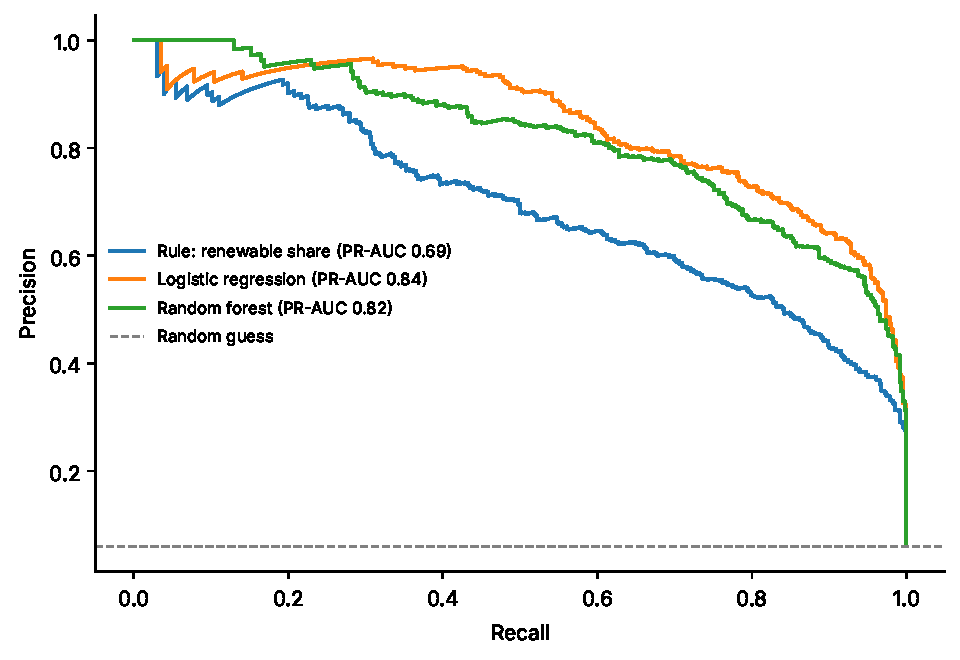
\includegraphics[width=0.5\textwidth]{figures/fig_pr_curves.pdf}
    \caption{Precision-recall curves of the negative-price classifiers on the test year 2026}
    \label{fig:pr}
\end{figure}

\section{Discussion} \label{sec:discussion}

\subsection{Why does the model ranking change in 2026?} \label{sec:ranking}

On the validation year, the random forest clearly outperformed the linear regression (12.97 vs.\ 14.55\,EUR/MWh). On the test year, the linear regression was slightly better (20.39 vs.\ 21.00). Figure~\ref{fig:monthly} shows that the ranking is not stable even within 2026. The random forest is the best single model in five months (January, February, April, June and November). The linear regression leads in five others (March, May, July, August and October), and the MLP in September.

Part of the explanation lies in the rise of the price level in autumn 2026. From January to August, the monthly mean price was between 79 and 127\,EUR/MWh. It then climbed to 145\,EUR/MWh in September, 169 in October and 245 in 1--17 November. From September on, the 30-day mean price was often higher than at any time in the two-year training window. This applied to 43\,\% (September), 98\,\% (October) and 94\,\% (November) of the hours. Tree models cannot extrapolate. Each leaf predicts an average of training observations, so their forecasts stay within the range of situations seen before. A linear model, by contrast, can extrapolate along price-level features such as \texttt{lag24} and \texttt{prev\_day\_mean}. Accordingly, the gap between the two is largest in October (26.2 vs.\ 31.0\,EUR/MWh).

\begin{figure}[!htbp]
    \centering
    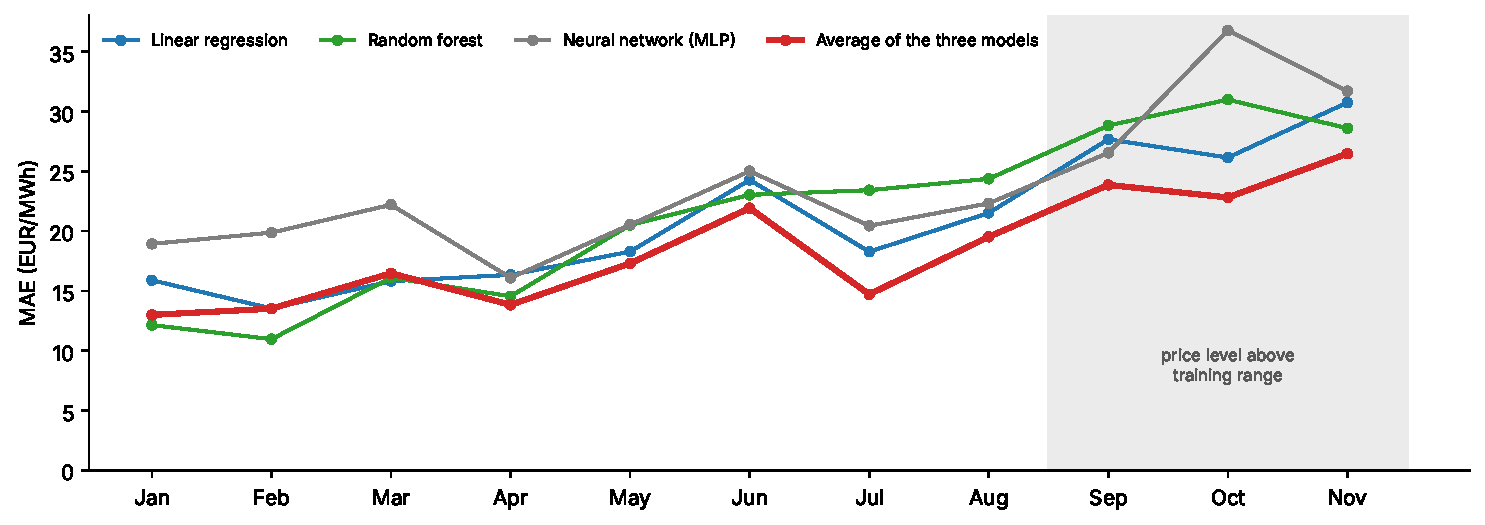
\includegraphics[width=\textwidth]{figures/fig_monthly_mae.pdf}
    \caption{MAE by month on the test year 2026; in the shaded months the price level was above the range of the training window}
    \label{fig:monthly}
\end{figure}

The average combines these properties. The random forest captures the non-linear merit order, and the linear regression follows shifts in the price level. The MLP, in turn, reacts strongly to extreme situations. The average is the best model in 8 of the 11 test months. In the other three, it is at most 2.6\,EUR/MWh behind the best single model. This is exactly the situation in which \citet{nowotarski2014} find equal-weight averaging to be a simple but powerful choice: no individual model consistently outperforms the others. For RQ2, we therefore draw a clear conclusion. In a changing market, the most robust strategy combines monthly retraining on two years of data with a simple average of different models.

\subsection{Error analysis}

\textbf{Bias towards the average.} Table~\ref{tab:bins} groups the test errors of the final model by the actual price. Figure~\ref{fig:errors} shows the error by hour of the day. The model overestimates low and negative prices and underestimates high prices. For prices above 300\,EUR/MWh, the mean error reaches 77\,EUR/MWh. Such regression towards the mean is typical when models minimize average errors and extreme hours are rare in the training data. The error is lowest at night (about 13\,EUR/MWh). It peaks in the evening hours 19:00--20:00 (about 25\,EUR/MWh), when the price reacts most strongly to the residual load.

\begin{table}[!htbp]
    \centering
    \caption{Errors of the final model by actual price range, test 2026 (error = actual $-$ forecast, EUR/MWh; each range includes its upper bound)}
    \begin{tabular}{lrrr}
        \toprule
        Actual price range & Hours & Mean error & MAE \\
        \midrule
        0 and below & 504 & $-3.7$ & 17.5 \\
        0 to 50 & 693 & $-6.6$ & 16.6 \\
        50 to 100 & 1,451 & 8.0 & 16.8 \\
        100 to 150 & 2,820 & 6.1 & 14.3 \\
        150 to 200 & 1,348 & 9.2 & 17.7 \\
        200 to 300 & 745 & 15.5 & 26.5 \\
        above 300 & 143 & 77.0 & 80.0 \\
        \bottomrule
    \end{tabular}
    \label{tab:bins}
\end{table}

\begin{figure}[!htbp]
    \centering
    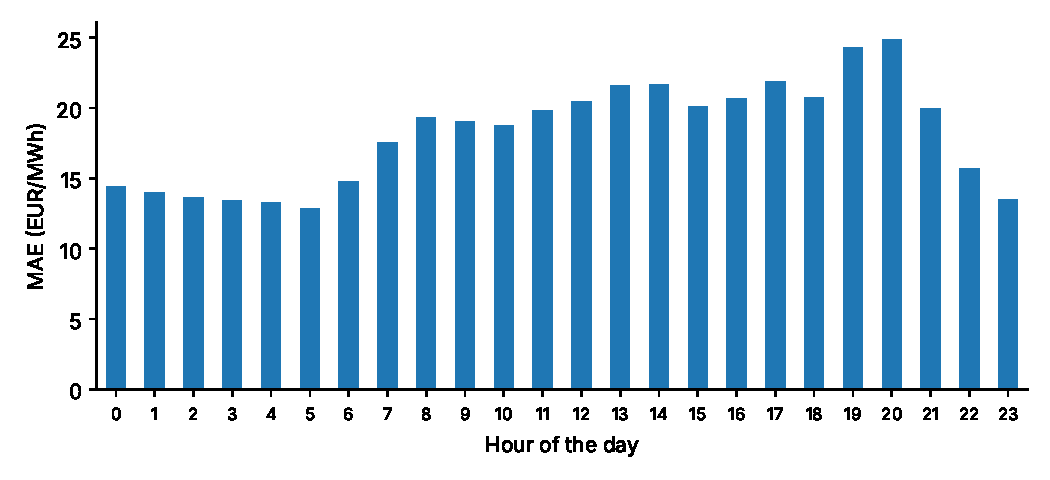
\includegraphics[width=0.7\textwidth]{figures/fig_error_analysis.pdf}
    \caption{MAE of the final model by hour of the day, test 2026}
    \label{fig:errors}
\end{figure}

\textbf{Example weeks.} Figure~\ref{fig:weeks} shows two weeks of the test period. In May 2026, the model follows the daily shape well, including the midday price drops caused by solar power. On the weekend of 9--10 May, it predicted clearly negative prices, down to about $-39$\,EUR/MWh. The actual price, however, stopped at about $-2$\,EUR/MWh. In November 2026, the model reacted to a period with little wind and sun (\enquote{Dunkelflaute}). Still, it underestimated the evening spike on 9 November. The actual price reached 644\,EUR/MWh at 17:00, while the forecast was 381\,EUR/MWh. The naive forecast reproduces every spike one day too late.

\begin{figure}[!htbp]
    \centering
    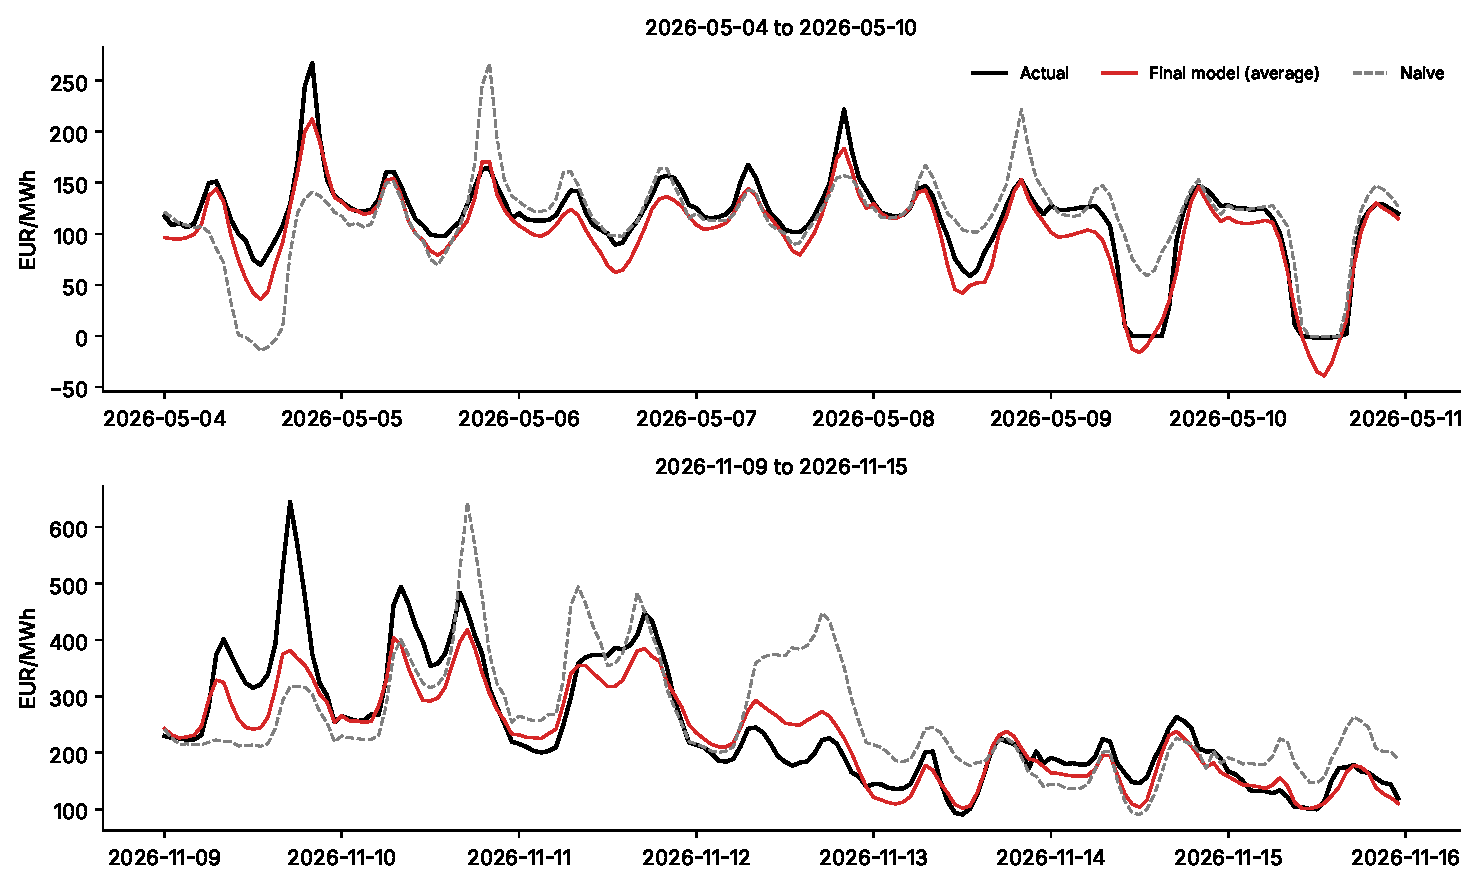
\includegraphics[width=\textwidth]{figures/fig_test_weeks.pdf}
    \caption{Forecast of the final model, naive forecast and actual price in two test weeks}
    \label{fig:weeks}
\end{figure}

\textbf{Worst days.} Four of the five days with the highest daily MAE had peak prices between about 500 and 670\,EUR/MWh. These were 24 June, 30 June, 29 October and 9 November 2026. The fifth was 1 May 2026, a public holiday with negative prices for most of the day (daily mean $-2.1$\,EUR/MWh). Such days depend on factors that the SMARD forecasts do not show directly, such as power plant outages, gas prices or cross-border flows.

\subsection{Which features drive the forecasts?}

Figure~\ref{fig:importance} shows the feature importance of the random forest trained on the latest two years of data. This measure captures how much each feature reduces the error inside the trees. The forecasted residual load is the most important feature. The renewable share and yesterday's price at the same hour (\texttt{lag24}) follow. Together, these three account for more than 60\,\% of the total importance. The price-level features (\texttt{same\_hour\_mean\_7d}, \texttt{mean\_30d}, \texttt{prev\_day\_mean}) come next. They tell the model how expensive the market currently is. Calendar features matter little once the residual load is known, since the residual load already contains the daily and weekly demand pattern. This importance measure favours features with many different values. It is therefore a rough guide rather than an exact ranking. The coefficients of the linear regression (notebook 02) point in the same direction. The largest positive effects come from \texttt{lag24}, the change of the residual load compared with the previous day and the previous day's mean price. The renewable share has a negative effect.

\begin{figure}[!htbp]
    \centering
    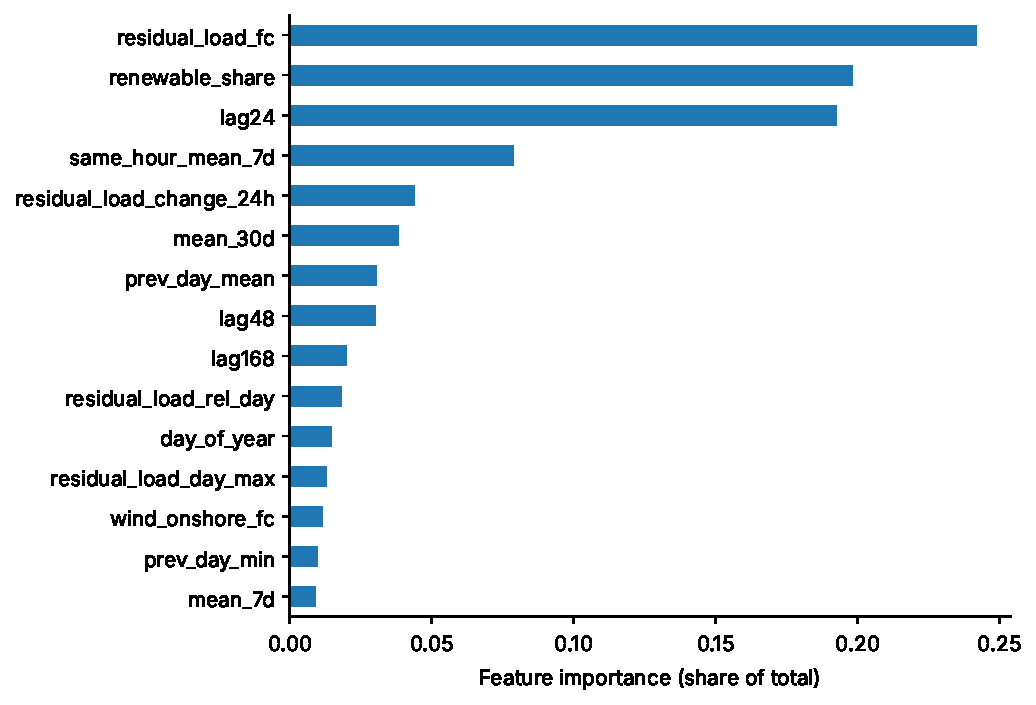
\includegraphics[width=0.62\textwidth]{figures/fig_feature_importance.pdf}
    \caption{Feature importance of the random forest (15 most important features, trained on November 2024 to November 2026)}
    \label{fig:importance}
\end{figure}

The partial dependence plot \citep{friedman2001} of the residual load (Figure~\ref{fig:pdp}) shows how the forecast changes when only the residual load varies. The curve has the step shape of the merit order. Below about 20\,GWh, the forecast falls steeply. Here, renewables push conventional plants out of the market and prices can become negative. Between 20 and 40\,GWh, the curve is flatter, as lignite and hard coal plants set the price. Above about 45\,GWh, it rises faster again, because expensive gas plants are needed. The model has learned this economic relationship from data alone. This answers RQ3 and increases the trust in its forecasts. A linear regression would describe the same relationship with a straight line.

\begin{figure}[!htbp]
    \centering
    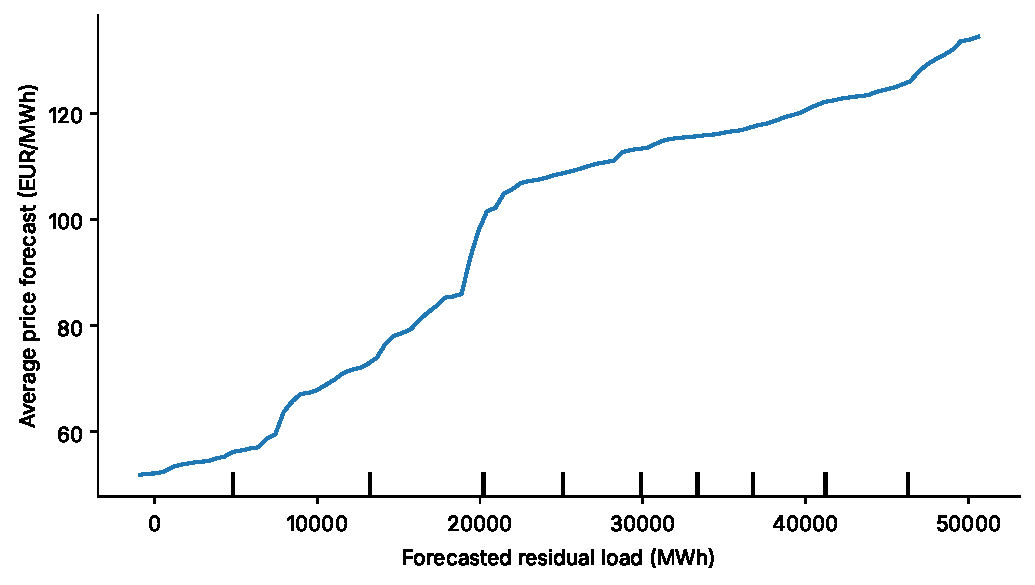
\includegraphics[width=0.6\textwidth]{figures/fig_partial_dependence.pdf}
    \caption{Partial dependence of the random-forest price forecast on the forecasted residual load (2,000 sampled hours of 2026): the learned merit-order curve}
    \label{fig:pdp}
\end{figure}

For the negative-price classifier, we examine the standardized coefficients of the logistic regression. Four conditions increase the probability of negative prices. They are a low residual load, a lower residual load than the day before, high solar forecasts and low prices on the previous day. High offshore wind has a negative coefficient once the other features are known. This reflects a correlation within the data and should not be read as a causal effect. Offshore wind is high mainly in winter nights with high demand and no solar power.

\subsection{Errors of the negative-price classifier}

The classification errors are economically small. False alarms have a median price of 5.2\,EUR/MWh. In these hours, the model correctly identifies an oversupply situation in which the price just stays positive. Missed hours have a median price of $-0.24$\,EUR/MWh. Negative hours occur almost exclusively between 9:00 and 17:00 from March to September. This pattern confirms that solar generation is the main driver. The threshold chosen on 2025 favours recall over precision. A battery operator who wants fewer false alarms could choose a higher threshold.

\subsection{Limitations} \label{sec:limitations}

\begin{itemize}
    \item \textbf{Missing fuel prices.} Gas and CO$_2$ prices drive the general price level, but the SMARD data does not contain them. Rolling price features and monthly retraining compensate for this only partly, as the higher errors in 2026 show.
    \item \textbf{Extreme prices.} The models are biased towards the average and underestimate spikes.
    \item \textbf{No systematic tuning.} The random forest and the MLP use common, fixed settings. Tuning them with time-series cross-validation might improve the single models. The averaging, however, already reduces the dependence on any one model.
    \item \textbf{Resolution.} We forecast hourly averages, while the market has traded 15-minute products since October 2025.
    \item \textbf{Publication time of the renewable forecasts.} The official wind and solar forecasts may be published after the auction closes (Section~\ref{sec:leakage}). Without any wind and solar information, the MAE of the final model rises to 29.38\,EUR/MWh (Section~\ref{sec:robust}). A forecaster with own weather-based forecasts would lie between this worst case and our main result.
    \item \textbf{Single market and period.} The results apply to Germany/Luxembourg and a test period of less than one year. They may differ for other markets or years.
\end{itemize}

\section{Conclusion} \label{sec:conclusion}

We built an end-to-end machine learning system that forecasts hourly German day-ahead electricity prices from official SMARD data. The system uses only day-ahead forecasts, past prices and calendar information, and only models from the course.

\begin{itemize}
    \item \textbf{RQ1 (accuracy):} All learned models clearly beat the seasonal naive forecast. The final model is the simple average of linear regression, random forest and neural network. It reaches a test MAE of 18.18\,EUR/MWh in 2026, 45.3\,\% below the naive forecast. It also wins significantly more test days than every other model. Without any wind and solar information, it would reach 29.38\,EUR/MWh, so the renewable forecasts are the most valuable input.
    \item \textbf{RQ2 (changing market):} Monthly retraining on a two-year window works better than one or three years. The best single model changes from month to month. The plain average of different models is the best model in 8 of 11 test months. It is also the most robust choice when the price level shifts.
    \item \textbf{RQ3 (drivers):} The forecasted residual load, the renewable share and yesterday's prices are the most important features. A partial dependence plot shows that the random forest learns the step-shaped merit-order curve from data.
    \item \textbf{RQ4 (negative prices):} A logistic regression detects 92.9\,\% of the negative-price hours in 2026 (PR-AUC 0.84). Most remaining errors occur at prices close to zero, where wrong decisions are cheap.
\end{itemize}

The main weakness is the underestimation of extreme price spikes, partly because the data lacks fuel and CO$_2$ prices. Several next steps look promising. One is hyperparameter tuning with time-series cross-validation. Others are forecasts of price ranges instead of single values and forecasting at the 15-minute resolution of the current market. Finally, a simple battery charging strategy could use the predicted probabilities of negative prices. Such a strategy would measure the economic value of the forecasts.

As a prototype, we implemented a Gradio dashboard (\texttt{app/dashboard.py}, Figure~\ref{fig:dashboard}). Users pick any day of the test period and compare the out-of-sample forecasts of all models with the actual prices. Three examples are one click away: a normal workday, a Sunday with negative prices and the spike of 9 November.

\begin{figure}[!htbp]
    \centering
    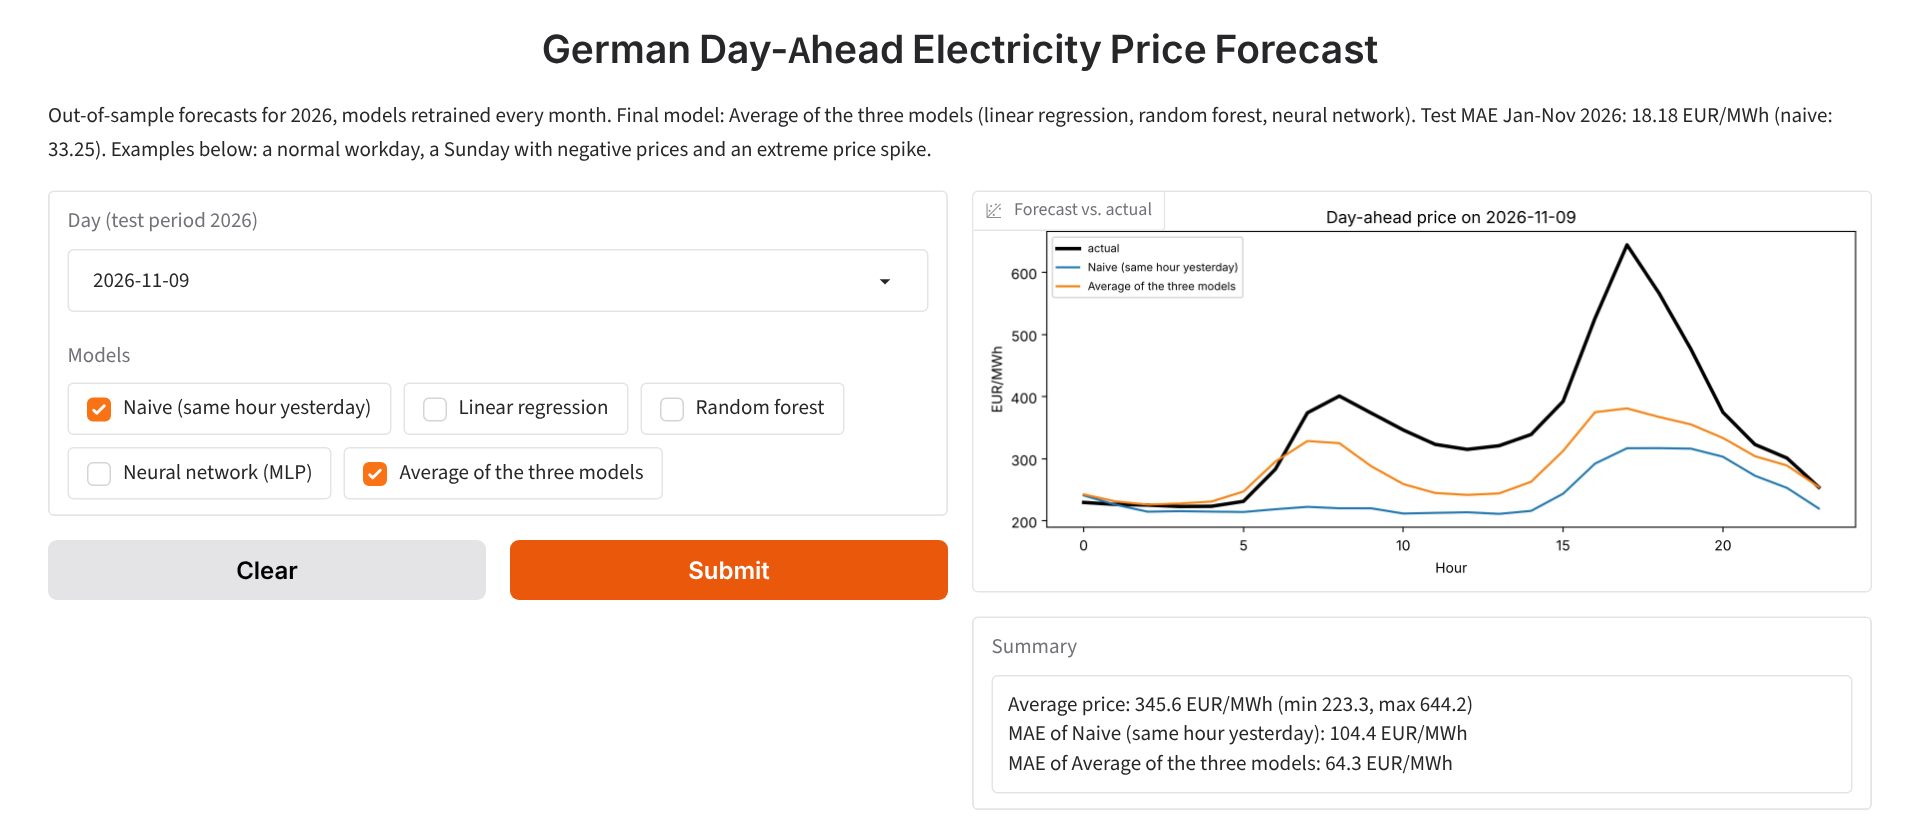
\includegraphics[width=0.85\textwidth]{figures/fig_dashboard.png}
    \caption{The Gradio dashboard showing 9 November 2026: actual price, naive forecast and final model}
    \label{fig:dashboard}
\end{figure}

\section{Use of Generative AI} \label{sec:genai}

As required, we document where we used generative AI and with which prompts. We used Claude (Anthropic) for the parts listed in Table~\ref{tab:genai}. % TODO group: check this table against what was actually done and add any further use.

{\small
\begin{longtable}{@{}>{\raggedright\arraybackslash}p{0.19\textwidth}>{\raggedright\arraybackslash}p{0.39\textwidth}>{\raggedright\arraybackslash}p{0.36\textwidth}@{}}
    \caption{Use of generative AI}\label{tab:genai}\\
    \toprule
    Part of the work & How AI was used & Main prompts (summarized) \\
    \midrule
    \endfirsthead
    \toprule
    Part of the work & How AI was used & Main prompts (summarized) \\
    \midrule
    \endhead
    \bottomrule
    \endlastfoot
        Topic selection & Suggested and compared possible topics based on the course requirements and the SMARD data & \enquote{With all the things you have please look at the data and tell us the most suitable topic for us}; \enquote{give me headlines for the topic proposals} \\
        \midrule
        Data download & Helped choose the SMARD download settings & \enquote{what is the choice for the period?} \\
        \midrule
        Project proposal & Drafted the two-page proposal & \enquote{with all the data we have create a proposal [\ldots] cover everything we should know} \\
        \midrule
        Code & Wrote the data pipeline, the three notebooks, the figure script and the dashboard in the style of the course notebooks; ran and checked them & \enquote{could you do a quick demo project using the way teacher codes in their lectures}; \enquote{why not just try the full version}; \enquote{do that, also make the code and report submittable} \\
        \midrule
        Simplification & Tested simpler versions, replaced the first version's gradient boosting (LightGBM), hyperparameter search, Diebold--Mariano tests and SHAP analysis with models and tools from the course, and re-ran all results & \enquote{I feel like this is way too advanced, we need something a bit simpler and easier to understand}; \enquote{do what you think is best, it shouldn't be worse just simpler} \\
        \midrule
        Report & Drafted this report from the notebook results and checked the references & \enquote{could you also write report for this code} \\
        \midrule
        Review and improvements & Checked all numbers against the notebook outputs and corrected errors (e.g.\ the publication time of the wind and solar forecasts, an inaccurate explanation of the model ranking); added the sign test, the monthly analysis and the robustness check; made the notebooks run in Google Colab and improved the dashboard & \enquote{Please look over again for fixes that needed, any mistakes that were not seen and things that can improve our grade and make our life easier}; \enquote{please look again this whole work, and just make it better} \\
        \midrule
        Presentation and team material & Created the slide deck with speaker notes, a project overview for the group (Word) and a private GitHub repository & \enquote{do the slide}; \enquote{also make a word file where I can show it to my teammates, so that they would understand it}; \enquote{I just want to connect my github to here and then you do everything else} \\
        \midrule
        Language revision & Revised the wording of this report for readability (shorter sentences, active voice, clearer transitions) without changing results, numbers, citations or the order of arguments & \enquote{use this prompt and edit the Report\_Forecasting\_German\_Day-Ahead\_Electricity\_Prices.pdf, make it a new file} (with a prompt for natural academic rewriting) \\
\end{longtable}
}

All numbers in this report come from running the submitted code. The group reviewed the code, the results and the interpretations. [To be completed by the group: what each member checked or changed.]

\section{Contributions of Group Members} \label{sec:contrib}

\begin{table}[!htbp]
    \centering
    \caption{Contributions of the group members}
    \begin{tabularx}{\textwidth}{lX}
        \toprule
        Member & Contributions \\
        \midrule
        Rashad Zarbaliyev & [e.g.\ topic selection, data download, proposal, coordination of code and report] \\
        {[Member 2]} & [e.g.\ exploratory data analysis, error analysis, presentation] \\
        {[Member 3]} & [e.g.\ model evaluation, negative-price classification, dashboard] \\
        \bottomrule
    \end{tabularx}
    \label{tab:contrib}
\end{table}



%%%%%%%%%%%%%%%%%%%%%%%%%%%%
%% The bibliography is inserted automatically
%%%%%%%%%%%%%%%%%%%%%%%%%%%%
\clearpage
\lhead{}
\printbibliography
\addcontentsline{toc}{section}{\bibname}


%%%%%%%%%%%%%%%%%%%%%%%%%%%%
%% Appendix
%%%%%%%%%%%%%%%%%%%%%%%%%%%%
\clearpage
\appendix
\section{Appendix A}

\subsection*{Code and reproducibility}

The submitted ZIP file contains the complete code (folder \texttt{code/}); its \texttt{README.md} explains installation and execution.

\begin{table}[!htbp]
    \centering
    \caption{Structure of the submitted code}
    \begin{tabularx}{\textwidth}{lX}
        \toprule
        File & Content \\
        \midrule
        \texttt{src/data\_pipeline.py} & Loading, cleaning, feature engineering, time split, monthly retraining loop \\
        \texttt{notebooks/01\_Data\_Preparation\_and\_EDA.ipynb} & Data quality checks and exploratory analysis (Section~\ref{sec:data}) \\
        \texttt{notebooks/02\_Price\_Forecasting\_Models.ipynb} & Baselines, models, training window, model selection, test evaluation, error analysis, feature importance \\
        \texttt{notebooks/03\_Negative\_Price\_Classification.ipynb} & Negative-price classification \\
        \texttt{src/report\_figures.py} & Creates all figures of this report \\
        \texttt{app/dashboard.py} & Gradio dashboard \\
        \texttt{outputs/} & Saved test predictions, result tables and feature importances \\
        \texttt{data/} & The four SMARD files \\
        \bottomrule
    \end{tabularx}
    \label{tab:code}
\end{table}

All random seeds are fixed (\texttt{random\_state=1}), so re-running the notebooks reproduces the numbers in this report. Notebook 02 runs in about 20 minutes on a standard laptop.

%%%%%%%%%%%%%%%%%%%%%%%%%%%%
%% Affidavit must be adapted
%% in declaration.tex
%%%%%%%%%%%%%%%%%%%%%%%%%%%%
%%%%%%%%%%%%%%%%%%%%%%%%%%%%
%% Declaration (affidavit), adapted for a group project
%%%%%%%%%%%%%%%%%%%%%%%%%%%%
\subsection*{Declaration}

We hereby declare that we have written this project report independently and have not used any sources or aids other than those indicated. All passages taken literally or in substance from other works have been marked as such. The use of generative AI is documented in Section~\ref{sec:genai}, stating the parts of the work for which it was used and the prompts. This report has not been submitted in the same or a similar form in any other examination procedure.

\vspace{1.5cm}

W\"urzburg, \rule{4cm}{0.4pt}

\vspace{1.5cm}

\begin{tabular}{p{4.5cm}p{4.5cm}p{4.5cm}}
\rule{4.2cm}{0.4pt} & \rule{4.2cm}{0.4pt} & \rule{4.2cm}{0.4pt} \\
Rashad Zarbaliyev & [Member 2] & [Member 3] \\
\end{tabular}


\end{document}
